\documentclass[border=4pt,varwidth=17cm]{standalone}
\usepackage{amsmath,amssymb,mathrsfs,mathtools}
\usepackage{tikz}
\usetikzlibrary{positioning,fit,backgrounds,arrows.meta}
\def\RR{{\mathbb R}}\def\eps{\varepsilon}\def\then{\Rightarrow}
\def\J{\mathcal{J}_L}\def\A{\mathcal{A}_{f,g}}\def\Sol{\mathcal{S}_{f,g}}
\def\limsup{\mathop{\overline{\lim}}}\def\liminf{\mathop{\underline{\lim}}}
\def\Of{{\sf (O$_f$)}}\def\Og{{\sf (O$_g$)}}
\def\Rv{{\sf (R$_{\rm v}$)}}\def\Rh{{\sf (R$_{\rm h}$)}}
\begin{document}


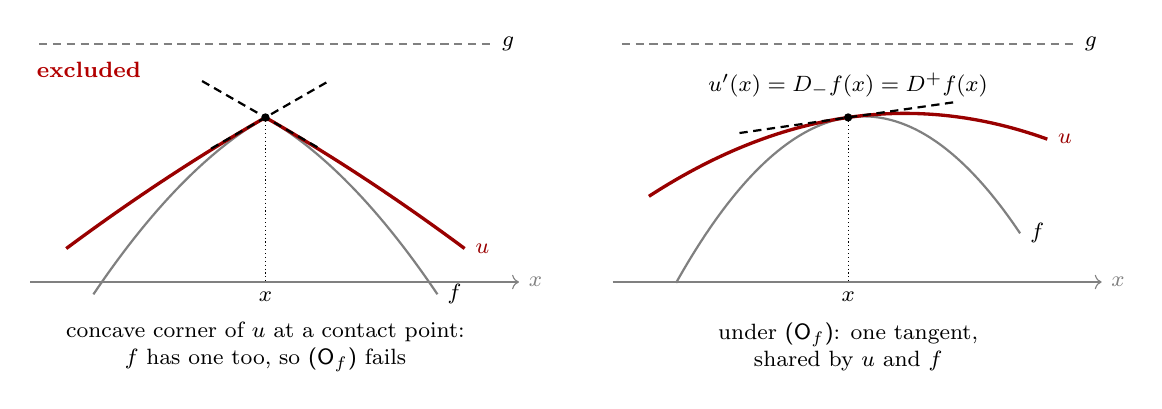
\begin{tikzpicture}[font=\footnotesize]
% left: excluded
\begin{scope}[x=1.15cm, y=1.1cm, declare function={U(\t)=1.9-0.6*abs(\t-2.5)-0.04*(\t-2.5)^2; F(\t)=1.9-0.6*abs(\t-2.5)-0.25*(\t-2.5)^2;}]
  \draw[->, gray] (-0.1,0) -- (5.3,0) node[right] {$x$};
  \draw[thick, gray, densely dashed] (0,2.75) -- (5,2.75) node[right, black] {$g$};
  \draw[thick, gray, domain=0.6:4.4, samples=60] plot (\x,{F(\x)}) node[right, black] {$f$};
  \draw[very thick, red!60!black, domain=0.3:4.7, samples=60] plot (\x,{U(\x)}) node[right] {$u$};
  \draw[thick, densely dashed] (1.9,{1.9-0.6*0.6}) -- (3.2,{1.9+0.6*0.7});
  \draw[thick, densely dashed] (1.8,{1.9+0.6*0.7}) -- (3.1,{1.9-0.6*0.6});
  \fill (2.5,1.9) circle (1.5pt);
  \draw[densely dotted] (2.5,1.9) -- (2.5,0) node[below] {$x$};
  \node[align=center] at (2.5,-0.75) {concave corner of $u$ at a contact point:\\ $f$ has one too, so \Of\ fails};
  \node[red!70!black, font=\bfseries\footnotesize] at (0.55,2.45) {excluded};
\end{scope}
% right: what remains
\begin{scope}[shift={(7.4,0)}, x=1.15cm, y=1.1cm, declare function={V(\t)=1.9-0.12*(\t-2.5)^2+0.15*(\t-2.5); G(\t)=1.9-0.45*(\t-2.5)^2+0.15*(\t-2.5);}]
  \draw[->, gray] (-0.1,0) -- (5.3,0) node[right] {$x$};
  \draw[thick, gray, densely dashed] (0,2.75) -- (5,2.75) node[right, black] {$g$};
  \draw[thick, gray, domain=0.6:4.4, samples=60, smooth] plot (\x,{G(\x)}) node[right, black] {$f$};
  \draw[very thick, red!60!black, domain=0.3:4.7, samples=60, smooth] plot (\x,{V(\x)}) node[right] {$u$};
  \draw[thick, densely dashed] (1.3,{1.9-0.15*1.2}) -- (3.7,{1.9+0.15*1.2});
  \fill (2.5,1.9) circle (1.5pt);
  \node[above] at (2.5,2.02) {$u^\prime(x)=D_-f(x)=D^+f(x)$};
  \draw[densely dotted] (2.5,1.9) -- (2.5,0) node[below] {$x$};
  \node[align=center] at (2.5,-0.75) {under \Of: one tangent,\\ shared by $u$ and $f$};
\end{scope}
\end{tikzpicture}


\end{document}
